%# -*- coding: utf-8-unix -*-
%%==================================================
%% chapter01.tex for SJTU Master Thesis
%%==================================================

%\bibliographystyle{sjtu2}%[此处用于每章都生产参考文献]
\chapter{大规模数据的索引建立}
\label{chap:c3}

在系统使用的完整的数据库中,论文的总量超过一亿两千万,因此索引建立的速度是建立方式选取的主要考量因素。由于论文数据库的内容在不断更新,随着时间的推移,数据库中会添加新的论文,现有论文的被引用量等信息也会改变,如果建立一次索引的时间过长,将会大大降低该系统的实时性与实用性。考虑到如果要在12小时内建立完整的索引,每秒导入条目的数量必须要大于2500条,这对建立索引的方法就有了很高的要求。经过多种方法的尝试后,本论文最终用文件导入法代替了之前的数据库导入法,成功将索引条目导入的速度从最初的每秒30条左右增加到了每秒4000条左右,成功做到了索引的实时建立与更新。

下面通过介绍并分析新旧两种导入方式,以解释这一问题的解决方式:
\section{数据库导入法}
数据库导入法是向Solr导入数据并建立索引的一种较为直观的方式,在Solr中的DataImportHandler包中有该方式的相关接口。由于数据源是MySQL数据库,因此导入过程采用JAVA提供的MySQL库中的jdbc.driver包进行驱动。

正如上一章中提到的,我们只要针对DataImportHandler包设计合适的db-data-config.xml文件,就可以实现数据库导入索引的操作。经过设计后,该文件的内容如下:
\begin{lstlisting}[caption={从数据库中导入索引的db-data-config.xml}, label=dbtoindex, escapeinside="", numbers=none]
<dataConfig>
    <dataSource type="JdbcDataSource"
      driver="com.mysql.jdbc.Driver"
      url="jdbc:mysql://*.*.*.*:**/database"
      user="******"
      password="******" />
    <document>
        <entity name="Papers" query="select * from Papers">
            <field column="PaperID" name="id" />
            <field column="OriginalPaperTitle" name="OriginalPaperTitle" />
            <field column="OriginalVenueName" name="OriginalVenueName" />
            <field column="PaperRank" name="PaperRank" />
            <field column="PaperPublishYear" name="PaperPublishYear" />
            <field column="ConferenceSeriesIDMappedToVenueName" name="ConferenceSeriesID" />
            <field column="JournalIDMappedToVenueName" name="JournalID" />
            <entity name="Information"
                    query="select * from PaperAuthorAffiliations
                    where PaperID='\${Papers.PaperID}'">
                <field name="AuthorID" column="AuthorID" />
                <entity name="Authors"
                  query="select AuthorName from Authors
                  where AuthorID = '\${Information.AuthorID}'">
                    <field name="AuthorName" column="AuthorName" />
                </entity>
            </entity>
            <entity name="Conference"
                    query="select ShortName from ConferenceSeries
                    where ConferenceSeriesID = '\${Papers.ConferenceSeriesIDMappedToVenueName}'">
                <field name="ConferenceShortName" column="ShortName" />
            </entity>
            <entity name="Keywords"
                    query="select * from PaperKeywords
                    where PaperID='\${Papers.PaperID}'">
                <field name="KeywordName" column="KeywordName" />
                <field name="KeywordID" column="FieldOfStudyIDMappedToKeyword" />
                <entity name="FieldsOfStudy"
                        query="select FieldsOfStudyName from FieldsOfStudy
                        where FieldsOfStudyID = '\${Keywords.FieldOfStudyIDMappedToKeyword}'">
                    <field name="FieldsOfStudyName" column="FieldsOfStudyName" />
                </entity>
            </entity>
            <entity name="PaperReferencesCount2"
                    query="select PaperReferenceCount from PaperReferencesCount2
                    where PaperReferenceID = '\${Papers.PaperID}'">
                <field name="PaperReferenceCount" column="PaperReferenceCount" />
            </entity>
        </entity>
    </document>
</dataConfig>

</requestHandler>
\end{lstlisting}

采用该方法,可以实现论文的顺利导入,经过实际测试,该方法可以在12小时内导入200万篇左右的文章。不过不幸的是,因为数据导入速度过慢,对于1.2亿条的数据,系统预计的导入时间超过了30天,而在服务器上将如此占用资源的进程连续运行30天是不可容忍的。由上一章可知,对于每一篇文章,需要索引的域共有14个,共涉及到数据库的七张表。由于该方法的索引建立的过程是逐条建立,而不是按表建立,因此需要通过表的连接(JOIN)方式将多张表的内容整合起来,再导入索引中。要整合得到所需的全部14个域,其中作者ID、会议简称、关键词名称、关键词ID需要进行一次表的连接操作;作者姓名、研究领域名称需要进行两次表的连接操作。由于大部分数据库表的规模很大,进行表的连接操作将会花费大量的时间。在实际操作中,使用该方法虽然可以完整建立功能完备索引,但是索引的速度只有每秒30条左右。考虑到服务器资源的限制与索引建立方式的可操作性,我们不得不抛弃这种方法,而寻找其它的解决方式。

\section{文件导入法}
在数据库导入法暴露了其致命缺陷之后,我尝试了很多改进方式,然而都没有从根本上解决这一问题。究其原因,是数据库表本身连接运算的效率过低导致的。在理论上,计算笛卡尔积的连接操作的复杂度达到了O(M*N),经过SQL内部优化的JOIN操作复杂度也在O(M+N)之上。由于这一部分涉及到大量硬盘读写,而硬盘的读写速度远远慢于内存与寄存器内的运算速度,这一典型的I/O密集型(I/O bound)工作的工作效率会被硬盘的读取速度大大限制。无论如何优化算法,或是给以程序更多的内存,只要读入数据的方式不改变,运行的速度就不会有本质上的提高。

弄清了问题的本质以后,改进该部分的重点就到了如何减少硬盘的读写上。其中一个可行的方式,也是论文中采用的方式,就是完全抛弃调用数据库操作处理数据,而将全部的数据操作都放在内存中的哈希表中进行,我把这种方法叫做文件导入法。该方法的核心,是先将数据库中的内容处理为XML格式的标记语言文件,再用该文件作为数据源建立索引。由于处理得到的文件中每条论文信息可以被逐条导入,因而这种方法完全避免了I/O密集的数据库操作,经过测试,使用该方法的导入速度相比数据库导入法提升了100-200倍,使大规模索引快速建立这一目标得到了实现。

文件导入法的第一步是将数据库中的数据重构为标记语言文件数据,算法描述如下:

\begin{itemize}
\item 链接数据库,选取与搜索平台需要索引的内容相关的表,将表中的内容导出到文件中;
\item 依次读入这些文件,用二级字典的形式保存文件内容。其中,字典的第一级为表的主键,字典的第二级为表的其它键,字典中保存的内容为表的键值;
\item 遍历保存Papers表的字典,用字典的查询操作代替数据库表的链接操作,扩展保存Papers表的内容。例如,当查询到论文作者的姓名后,即在Papers字典的二级键中加入一个名为AuthorName的键,并保存相应的键值;
\item 将扩展完整的Papers字典保存为xml文件,为了后续引用方便,此处文件命名为transed\_all.xml。
\end{itemize}

该算法先将数据库保存到文件中,再读入文件建立字典,而不是直接从数据库建立字典。这是因为数据库的多行导出比逐行导出的速度要快很多,因此这里不将数据库逐行导出到字典,而是添加了一个中间步骤。

在按此方法从数据库读取并重构了数据之后,我们得到的transed\_all.xml文件便以逐条呈现的形式存储了所有需要被索引的信息。此时我们以该xml文件为数据源进行索引创建的时候,就可以避免耗时的数据库读取与链接操作,而可以通过顺序读文件的方法完成索引的建立。此时,db-data-config.xml的配置也会变得简单很多。注意,此时要以流形式(stream = true)导入数据,可以让系统逐行读取目标文件,避免文件过大导致资源不足。

\begin{lstlisting}[caption={从文件导入索引的db-data-config.xml}, label=filetoindex, escapeinside="", numbers=none]
<dataConfig>
	 <dataSource encoding="UTF-8" type="FileDataSource" />
	 <document>
	    <entity
	        name="paper"
			processor="XPathEntityProcessor"
			forEach="/root/paper"
			url="/foo/bar/transed\_all.xml"
			stream="true"
			>
		<field column="id" xpath="/root/paper/PaperID" />
		<field column="OriginalPaperTitle" xpath="/root/paper/OriginalPaperTitle" />
		<field column="OriginalVenueName" xpath="/root/paper/OriginalVenueName" />
		<field column="PaperRank" xpath="/root/paper/PaperRank" />
		<field column="PaperReferenceCount" xpath="/root/paper/CitationCount" />
		<field column="PaperPublishYear" xpath="/root/paper/PaperPublishYear" />
		<field column="ConferenceSeriesID" xpath="/root/paper/ConferenceSeriesIDMappedToVenueName" />
		<field column="JournalID" xpath="/root/paper/JournalIDMappedToVenueName" />
		<field column="ConferenceShortName" xpath="/root/paper/ConferenceShortName" />
		<field column="AuthorID" xpath="/root/paper/Author/AuthorID" />
		<field column="AuthorName" xpath="/root/paper/Author/AuthorName" />
		<field column="AuthorSequenceOrder" xpath="/root/paper/Author/AuthorSequenceOrder" />
		<field column="FieldsOfStudyName" xpath="/root/paper/Keyword/FieldsOfStudyName" />
		<field column="KeywordID" xpath="/root/paper/Keyword/KeywordID" />
		<field column="KeywordName" xpath="/root/paper/Keyword/KeywordName" />
    </entity>
    </document>
</dataConfig>
</requestHandler>
\end{lstlisting}

该导入配置文件比数据库导入法的配置文件要简单很多。这是因为,此时需要导入的内容都在xml树的同一个根节点下平铺展开,所以只需要顺序读入该文件的xml树并获取对应域的内容,就可以完成文档的导入工作。

这是一个典型的用空间换时间的算法,其本质为将硬盘中的内容映射到内存中,再利用内存比硬盘高得多的读写速度完成任务。这种空间换时间以提高效率的方法在本平台中也有许多其它的运用场景。如论文2.5章中谈到的,在索引的构建过程中,如果将60G的索引文件映射到内存中,并直接在内存上执行索引查询请求,会使查询的速度相比于将索引存放于文件中大大提高。但是在服务器中,内存空间是一种比磁盘空间宝贵的多的资源,长时间占用60G-120G(60G为单机版索引总大小,120G为分布式索引总大小)的内存资源也是一项很大的花费。因此,这种方法的使用需要经过慎重考虑。

\section{两种导入方式的性能对比}

我们在单机版服务器上对两种导入方式的速度进行了测试,如图\ref{fig:dim}所示,我们可以在数据导入监视器上查看当前的数据导入情况。图中可以看出,当前的索引建立速度为每秒钟4025条,我们当前已从数据源处取来了108,681条数据,其中的108,680条数据已经被成功建立索引。这是一次文件导入法开始约30秒后的截图,此时索引的建立速度很快。

\begin{figure}[!htp]
  \centering
  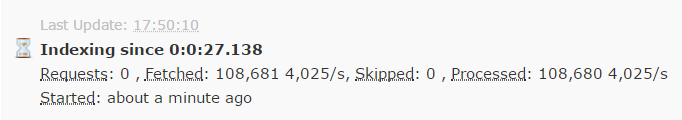
\includegraphics[width=0.7\textwidth]{dataimportmonitor.png}
  \bicaption[fig:dim]{数据导入监视器}{数据导入监视器}{Fig}{data import monitor}
\end{figure}

如图\ref{fig:dfc}所示,我们分别用数据库导入法和文件导入法建立索引,并在索引开始第1小时,第2小时,第8小时和第40小时的时刻记录当前数据导入监视器上的索引建立速度。重复进行三次实验取速度的平均值,可以得到两种导入方式的对比折线图。

\begin{figure}[!htp]
  \centering
  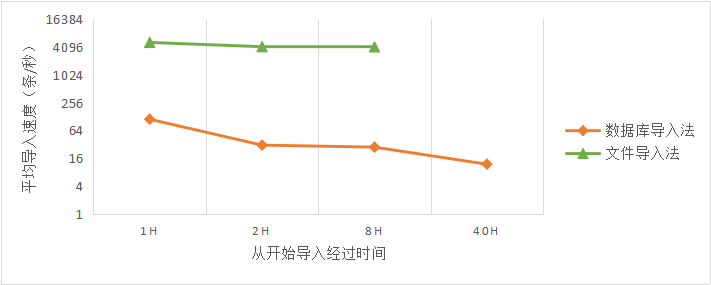
\includegraphics[width=0.75\textwidth]{dfc.png}
  \bicaption[fig:dfc]{两种导入方式的对比}{两种导入方式的对比}{Fig}{file import and database import}
\end{figure}

从表格中我们可以观察到,当索引导入开始时,文件导入法的导入速度超过每秒4000条,数据库导入法的速度约为每秒钟100条,此时文件导入法的导入速度是数据库导入法的40倍。当索引导入进行到第8小时的时候,文件导入法的导入速度仍然稳定在每秒4000条左右,而此时数据库导入法的速度已不到文件导入法的百分之一。在第40小时的时候,文件导入法早已进行完毕,而数据库导入法的数据导入过程还在以每秒十条左右的速度缓慢进行。我们可以发现,相比于文件导入法,数据库导入法不仅导入速度慢,而且其导入速度随时间衰减的现象也较之文件导入法更为严重。事实上,两种导入方式最本质的区别在于数据导入形式的区别,从这个角度,我们分析此现象的原因如下:

\begin{itemize}
\item 在数据导入阶段,文件导入法只进行了读取文件流的操作,数据库导入法进行了连接数据库,发送表连接请求,等待服务器应答,接收数据四个阶段。而在等待数据库服务器应答阶段,索引服务器将会花费大量的时间在等待服务器进行表连接操作上,在这一阶段中索引服务器处于空闲状态。因此,数据库导入法的速度相对于文件导入法会慢很多。
\item 在数据导入进行过程中,文件导入法每次只处理读入的当前文件流,之前读入到内存的数据在处理完成后可以直接销毁;而在数据库导入法中,数据库服务器的运行速度会随着时间的推移产生越来越多的缓存,运行速度也会越来越慢,此时,索引服务器在等待每次表连接操作时会等待更长的时间。因此,文件导入法的速度随时间变化的波动不大,而数据库导入法的导入速度会随着时间推移严重衰减。
\end{itemize}